\documentclass[fleqn,12pt]{olplainarticle}
\usepackage{graphicx}
\graphicspath{ {./} }
% Use option lineno for line numbers 
\renewcommand{\baselinestretch}{1.3}

\title{Docker in Software Architecture – Technology brief (c)}

\author[1]{Daniel Koch}
\author[2]{Sebastian Sergelius}
\affil[1]{daniel.koch@helsinki.fi}
\affil[2]{sebastian.sergelius@helsinki.fi}

\keywords{docker, software architecture, containers}

\begin{abstract}
Docker is currently very popular in software development and software deployment. It promises many advantages that are relevant in modern
software development, like scalability, maintainability, security, and portability. In this report, we study the architecture of Docker as well as Docker's
architectural impact on software development.
Writers are defined with initials on sections and/or subsections.
\end{abstract}

\begin{document}
\flushbottom
\maketitle
\thispagestyle{empty}
\pagebreak
\tableofcontents
\section{Introduction (DK/SS)}

With the rise of DevOps and the use of Docker, containerization has become more and more relevant to think about even in software architecture. DevOps does not have any official definition.
One formal definition is given by \cite{Jabbari_devops}: 
\begin{displayquote}
"DevOps is a development methodology aimed at bridging the gap between Development and Operations, emphasizing communication and collaboration, continuous integration, quality assurance and delivery with automated deployment utilizing a set of development practices".
\end{displayquote}
Another way to put DevOps is that it consists of the development of software and operations and that DevOps means that development, release, configuration, and monitoring are all done by the same people, rather than having separate teams for every part \citep{hy:DevOps_with_Docker}.

Containerization is common as a part of DevOps. Docker is one of the most common containerization software since its release in 2013 \citep{aquasec:orchestration}. Docker is a product that enables you to easily develop, ship, and run your application on different infrastructures by using OS-level virtualization \citep{docker:overview}. In this technology brief, we will explain what is meant by containerization, how it compares to virtual machines and how do you use docker as a part of software architecture. 

We will start by comparing Docker and Virtual Machines in chapter 2. In chapter 3 we examine the technical components of the thing under study. Chapter 4 describes the qualities that Docker has hoisted in it followed by the architectural impact in chapter 5. In chapter 6 we will discuss some limitations when using Docker and limitations within its qualities. Chapter 7 will be about some of the most common Docker tools and orchestration frameworks and shortly about their advantages. Chapter 8 will be a conclusion.

\section{Docker containers and virtual machines (DK)}

Virtualization is a much older technology than Docker and virtual machines have been used for decades. To understand Docker a bit better, we need to compare
it to virtual machines because it is important to understand that Docker is not the same thing as a virtual machine. We can see the largest difference between Docker and virtual machines in Figure \ref{fig:dockervsvm}: Virtual machines always have their own Guest OS, but Docker does not. This means that with every virtual machine we need to ship a complete OS with them, but Docker uses the underlying OS through the Docker Engine. Therefore, shipping multiple Docker containers is much lighter than shipping multiple virtual machines. However, virtual machines give you more freedom and easier configurability. In real-world cases, they are usually used together in cloud environments: The client has a virtual machine on the cloud and runs multiple Docker containers on the virtual machine.

The Docker product uses many features from the Linux kernel for delivering OS-level virtualization, the most important ones being namespaces and control groups \citep{docker:security}. Kernel namespaces provide isolation for containers so that they can not affect other processes running on the host machine or in another container. Control groups are used for creating a fair share of computational resources for each container running on the host machine. Control groups also make sure that a container can not crash the host machine by overusing computational resources, such as disk I/O, memory or CPU. Each container also has its own network stack, so it can not access other containers' sockets and interfaces.

\begin{figure}[h]
    \centering
    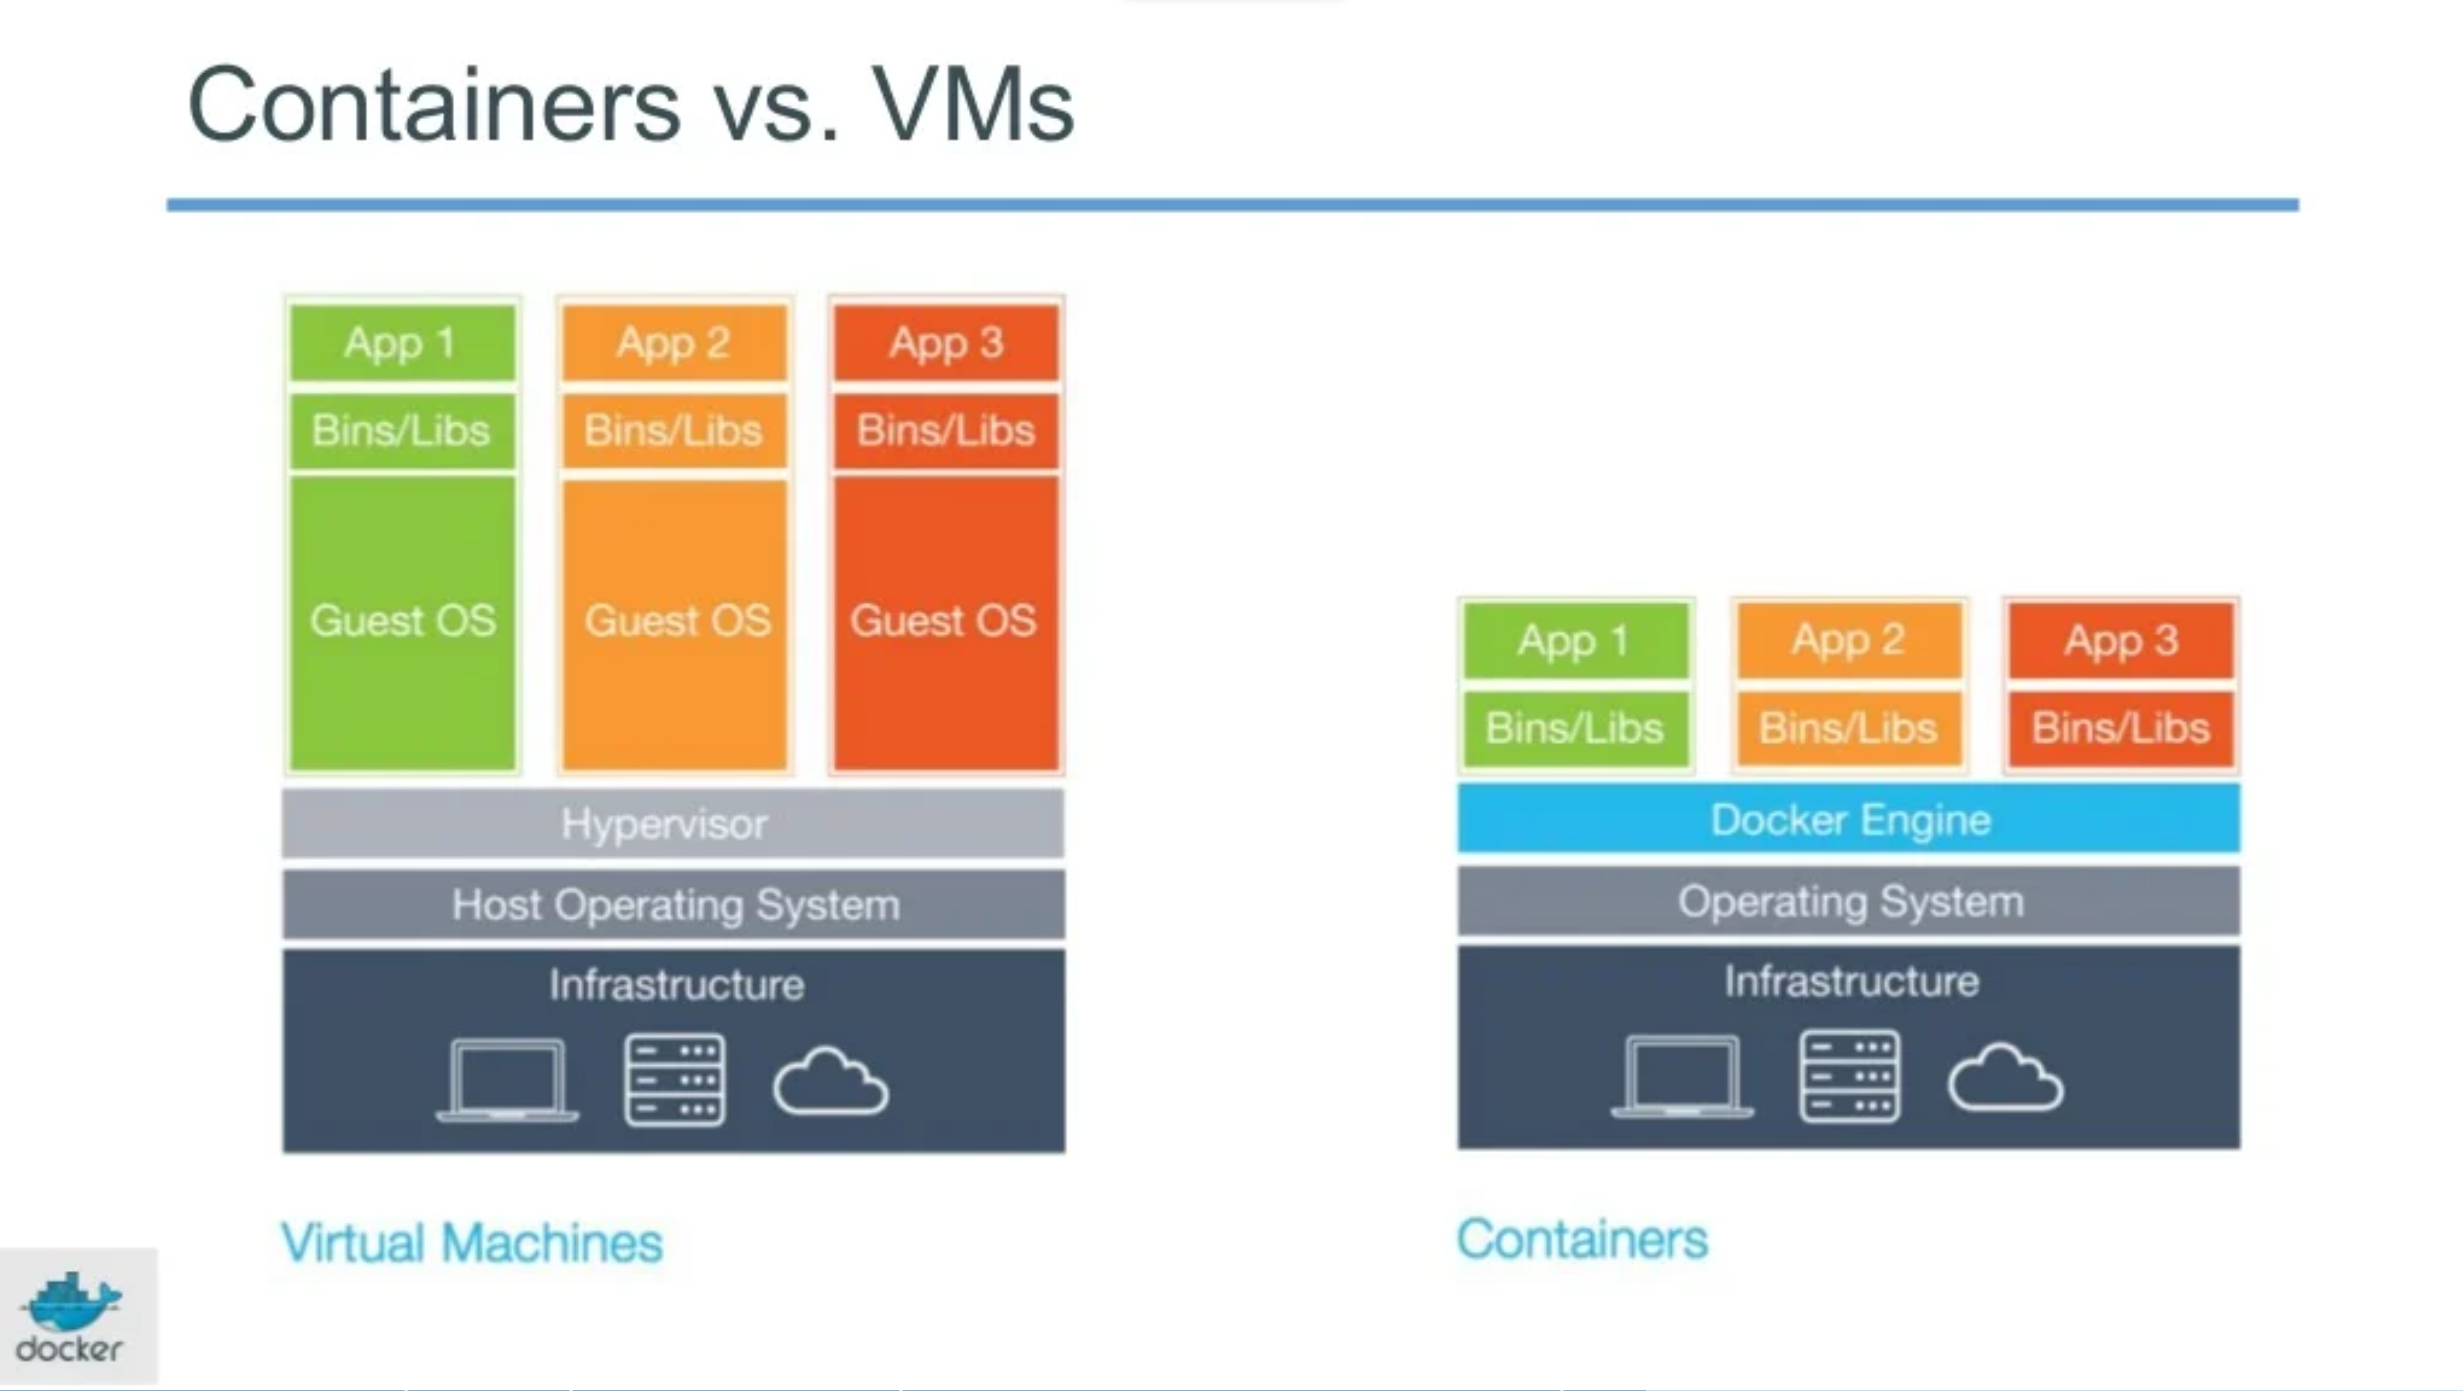
\includegraphics[width=1\textwidth]{docker_vs_vm.png}
    \caption{Docker vs. virtual machines \cite{docker:vs_vm}}
    \label{fig:dockervsvm}
\end{figure}

\section{Docker Architecture (SS)}

In this section, we will be discussing the Docker architecture and its vital components that build the technology under study. The Docker architecture is based on a client-server model where the client is called Docker client and the server is called Docker Host, see Figure \ref{fig:overview} \citep{docker:overview, aquasec:docker_architecture}. The client and the host do not necessarily need to be on the same system, as the client can communicate with the host using the Docker REST API through either a UNIX socket or a network interface. Docker images are specified in a Dockerfile, which defines the steps of how to build and run the image in a container. These built images can be stored in a private or public Docker Registry.

\begin{figure}[h]
    \centering
    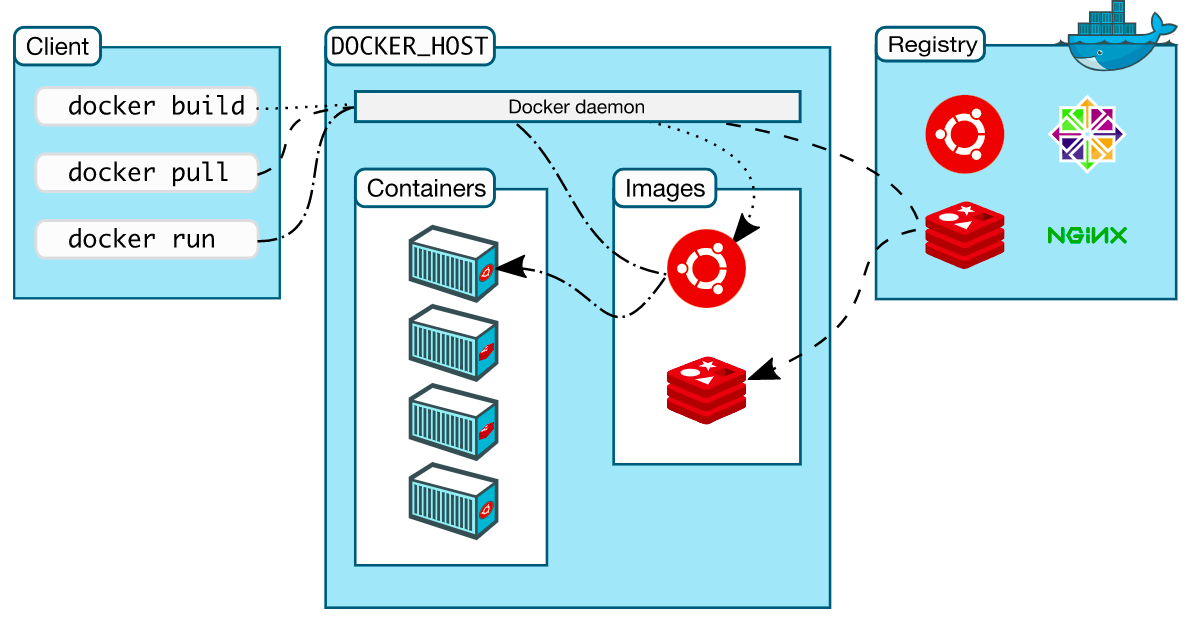
\includegraphics[width=1\textwidth]{docker-overview}
    \caption{Overview of the Docker Architecture where we can see the vital components (Client, Host, and Registry) and the sub-components they provide \citep{docker:overview}}
    \label{fig:overview}
\end{figure}

\subsection{Docker Client}

The Docker Client is the application that the user uses to interact with the Docker environment \citep{aquasec:docker_architecture}. The client provides a command-line interface (CLI) that enables the user to give commands to the Docker Hosts daemon. A client is able to communicate with many daemons.

\subsection{Docker Host}

The Docker host contains many components, such as the daemon, images, containers, networking, and storage, that provide the environment for running and executing applications \citep{aquasec:docker_architecture}. The daemon is responsible for handling container-related commands that are received from the client, such as pulling pre-built images from a registry, executing instructions defined in a Dockerfile, and building and running the containers on the server.

\subsubsection{Docker Images}

Docker Images are read-only binary files that are used to build containers \citep{docker:overview}. Images are built using a Dockerfile that defines the instructions for the daemon to execute. Each instruction creates a layer in the image built. A layer can be thought of as a small image inside the larger image that is being built. If an instruction is changed in the Dockerfile the daemon will only rebuild the image on the layers affected by the change, thus speeding up the process of creating containers from slightly modified images. Once the image is built, you can run the image in a container. Each container can be saved as an image and images support versioning.

\subsubsection{Docker Containers}

Docker Containers are isolated environments that run applications \citep{aquasec:docker_architecture}. The container contains all the necessary dependencies that are required for running the application. Running containers are isolated from other containers and also have good isolation from the host machine \citep{docker:security}. Containers are temporary and once they are deleted all the data within the container will disappear. Containers can be connected to a network and persistent storage.

\subsubsection{Docker Networking}

Docker uses \textit{iptables} rules on Linux hosts to provide network isolation \citep{docker:iptables}. Linux iptables provide the possibility to restrict access for the Docker host, as by default, all external IPs are able to connect to a Docker host. Docker environment has several network drivers by default, such as \citep{docker:network}:

\begin{itemize}
    \item \textbf{bridge}: The default driver. Used when multiple containers on the same host need to communicate with each other.
    \item \textbf{host}: Containers use the Docker host's networking layer directly.
    \item \textbf{overlay}: Used to connect multiple Docker daemons together. Should be used if two containers are on different Docker hosts.
    \item \textbf{none}: Disables container networking.  
\end{itemize}

Docker also supports third-party network plugins, user-defined IP addressing, and defining a MAC address to a container, so the container can be seen as a physical host in the network \citep{docker:network}.

\subsubsection{Docker Storage}

Data stored within the container are non-persistent and the data will disappear once the container stops running \citep{aquasec:docker_architecture}. For persistent storage, Docker offers four options – Data Volumes, Data Volume Container, Directory Mounts, and Storage plugins. 

Data volumes are located on the host's file system and can be shared with many containers. A data volume container is a dedicated container that hosts a volume from the host. Each container using the volume connects to the container that hosts the persistent storage. Using Directory mounting, a container can have access to any folder on the host and with storage plugins, containers can use persistent storage that is for example hosted on the cloud.

\subsection{Docker Registry}

A Docker registry is a service for storing and downloading images \citep{aquasec:docker_architecture}. A registry can be publicly or privately hosted. Some most known public registries are Docker Hub and Docker Cloud.

\section{Quality Attributes}

Based on how Docker is built, the system has some qualities hoisted in it. In this section, we will list some important qualities from the architectural and agile perspective, if you decide to use Docker in your infrastructure. 

\subsection{Portability (SS)}
One key aspect of Docker is its Portability. With software portability, we refer to the usability of the same software in different environments, such as the underlying operating system or hardware \citep{wiki:Software_portability}. Portability is achieved based on how the Docker technology is built. Each container includes all the dependencies required for the application to work and only requires an underlying operating system and infrastructure that supports the Docker Engine \citep{hy:DevOps_with_Docker}.

\subsection{Deployability (SS)}
As Docker images are versionable, this gives the possibility to easily test, roll back and deploy applications\citep{hentsu:benefits}. As Docker images are smaller than Virtual Machine images, deploying an image to production is fast and results in a short downtime when deploying to a production environment. 

\subsection{Security / Isolation (DK)}
Docker promises some security advantages if configured correctly \citep{docker:security}:
\begin{itemize}
    \item  Docker namespace is isolated from other programs on the machine. It cannot access other software namespaces and other software cannot access Docker's namespaces. 
    \item Each container has its own network stack and doesn't get privileged access to other containers' sockets.
    \item Docker utilizes control groups. For security, this means that a single container cannot bring the machine down even if it tried to. (Performance wise)
\end{itemize}

\subsection{Scalability (DK)}
Scalability is one of the main selling points of Docker and especially if bundled with microservice architecture the scalability is great. With Docker, you can easily deploy as many containers of your service as you need and even adjust the number of containers during runtime.

\subsection{Maintainability (DK)}
Docker separates all applications into their own virtual environments. With this, different applications don't interfere with other applications and each application can have all its dependencies easily and reliably every time without affecting other software. This allows different applications to use different versions of the same dependencies.

\subsection{Resiliency (DK)}
Docker brings good resiliency/recoverability to software. If a new version of the software has problems in production, it is easy to just roll back to the old 
container that was working without problems. Redeploying containers is also easy if something in the container crashes.

\section{Architectural impact (DK)}

Docker is mainly a tool for development and deployment. The application itself doesn't necessarily know if it is run on a physical machine, a virtual machine, or in a Docker container. Therefore, Docker does not absolutely have any impact on the software architecture. However, Docker excels with running multiple containers at the same time easily and therefore is a great tool for developing and deploying software with microservices architecture. This leads to the fact
that constructing microservices software becomes much less cumbersome and more easily configurable, so Docker allows people to make microservices more easily, making it a great pattern to develop and test and thus has an indirect architectural impact.

Docker ensures that the software is isolated from other software. This means that we don't have to think about how other software running on the same namespace or file system could affect our software nor how our software could affect other software or other parts of itself. This also makes the software more secure.
In addition, since every part of the software is run in its own virtual environment, the container, we can have different parts of the software use different versions of the same dependencies.

For development, since every dependency is defined in the image and is run within the container, everybody should have exact same development environment as what is used in production. This prevents bugs that happen because people have different configurations on their own machines which leads to "works on my machine" situations.

\section{Limitations (SS)}

As Docker adds a layer between the container and the host kernel it doesn't suit well if you need to get full performance from your underlying hardware, although it is still more lightweight than VMs \citep{cloudsavvy:not_to_use}. In comparison to virtual machines, containers are not able to run different operating systems that would require a different kernel than the underlying host machine. 

For simple monolith architectures and desktop applications with high graphical requirements, Docker containerization does not offer the possible qualities that the Docker orchestration and containerization provide. Although, portability might be something that is great to have in development of simple monolith architectures so that you can easily setup the development environment for your team.

As a user of the Docker environment, your configurations ensures that security and isolation is achieved with Docker. This can be achieved by always keeping the Docker Engine version up to date \citep{aquasec:docker-security-best-practices}. For configuration, you should try to run Docker in rootless mode and avoid running containers in privilege mode, this way you can mitigate the risk that the container could wrongly access the host or other containers. Trying to minimize the amount of dependencies within the container will also lower the attack surface. If you decide to use a base image from a Docker Registry, you should always study the image and ensure that it doesn't contain anything out of the ordinary.

Docker provides good isolation and security if the user knows what they are doing, this way one could say that Docker does not exactly hoist security and isolation when starting to use Docker out-of-the-box. This is a limitation that can be overcome by studying Docker and its caveats.

\section{Docker Tools (SS)}

Docker Engine is available on the common operating system, such as Windows, macOS, and Linux distributions, and on the most common processor architectures, i.e. x86\_64, amd64, arm, and aarch64 \citep{docker:install}.  On Windows and Mac, the Docker toolset that contains all the necessary components to run Docker is called Docker Desktop. Currently, for Linux, they are developing this same toolset as well. With the help of Docker tools, developers are able to run, terminate, build and manage images and containers easily without the need to install any additional programs to run an application on their local machine.

Docker Desktop for Windows uses the Windows Subsystem for Linux 2 (WSL2) or Hyper-V Hypervisor and Windows Containers feature, which is available on the most recent versions of 64-bit Windows 10 and 11 \citep{docker:windows}. In both cases you will have the Linux kernel running on top of the Windows operating system, either in a virtual machine or the more lightweight WSL2. 

For managing multiple containers in production you can use a container orchestration framework \citep{circleci:swarm_kubernetes}. The most common orchestration framework tools are Docker Swarm and Kubernetes. Orchestration tools provide some important features, for example, load balancing, scaling, availability, and self-healing of containers. Compared to Kubernetes, Docker Swarm is more lightweight but has fewer features. With the use of orchestration frameworks, you have less to worry about when having your software architecture deployed in production.

Another popular tool that is widely used for defining and running multi-container environments is Docker Compose. With help of Docker Compose you can spin up the whole multi-container environment with just one command, making it suitable for development environment, but works as well in production, staging, testing and CI/CD pipelines \citep{docker:compose-overview}. Some of the features that makes Docker Compose great is that it can run multiple isolated environments on the same host and it preserves volumes used by you environment, that is, it can copy volumes from old containers to the newly started containers.

\section{Conlusion}
Coming soon
\bibliography{sample}

\end{document}